\documentclass[12pt]{article}
\parindent=.25in

\setlength{\oddsidemargin}{0pt}
\setlength{\textwidth}{440pt}
\setlength{\topmargin}{0in}

\usepackage{amsmath}
\usepackage[dvips]{graphicx}
\usepackage{verbatim}
\usepackage{appendix}

\usepackage{amssymb}
\usepackage{amsfonts}
\usepackage{latexsym}
\usepackage[center]{subfigure}
\usepackage{epsfig}
\usepackage{hyperref}

\title{Stat 4201 Homework 7}
\author{Mengqi Zong $<mz2326@columbia.edu>$}

\begin{document}

\maketitle

% no paragraph indentation
\setlength{\parindent}{0in}

\section*{Question 1}

a) \\

The F-test shows that there is a significant difference among the
group means. Here is the output from R:

\begin{verbatim}
            Df  Sum Sq  Mean Sq F value   Pr(>F)   
Disease      2 0.43282 0.216411  7.9493 0.002522 **
Residuals   22 0.59892 0.027224                    
---
Signif. codes:  0 ‘***’ 0.001 ‘**’ 0.01 ‘*’ 0.05 ‘.’ 0.1 ‘ ’ 1 
\end{verbatim}

Now we try to calculate the  simultaneous confidence interval of
Bonferroni Method. Here is the output from MATLAB:

\begin{verbatim}
    'Controls'     [1]    [2]    [-0.3858]    [-0.1781]    [ 0.0297]
    'Gallstone'    [1]    [3]    [-0.5258]    [-0.3181]    [-0.1103]
    'Ulcer'        [2]    [3]    [-0.3538]    [-0.1400]    [ 0.0738]
\end{verbatim}

As we can see, the only confidence interval that does not contain zero
is Conrtols-Ulcer: $[-0.5258, -0.1103]$. This indicates that the means
of Controls and Ulcer are different. \\

b) \\

For the normality assumption, we use q-q plot of residuals to do
the analysis. The plot is shown in Fig-\ref{fig:qq}. As we can see,
the normality assumption holds.

\begin{figure}[ht!]
  \centering
  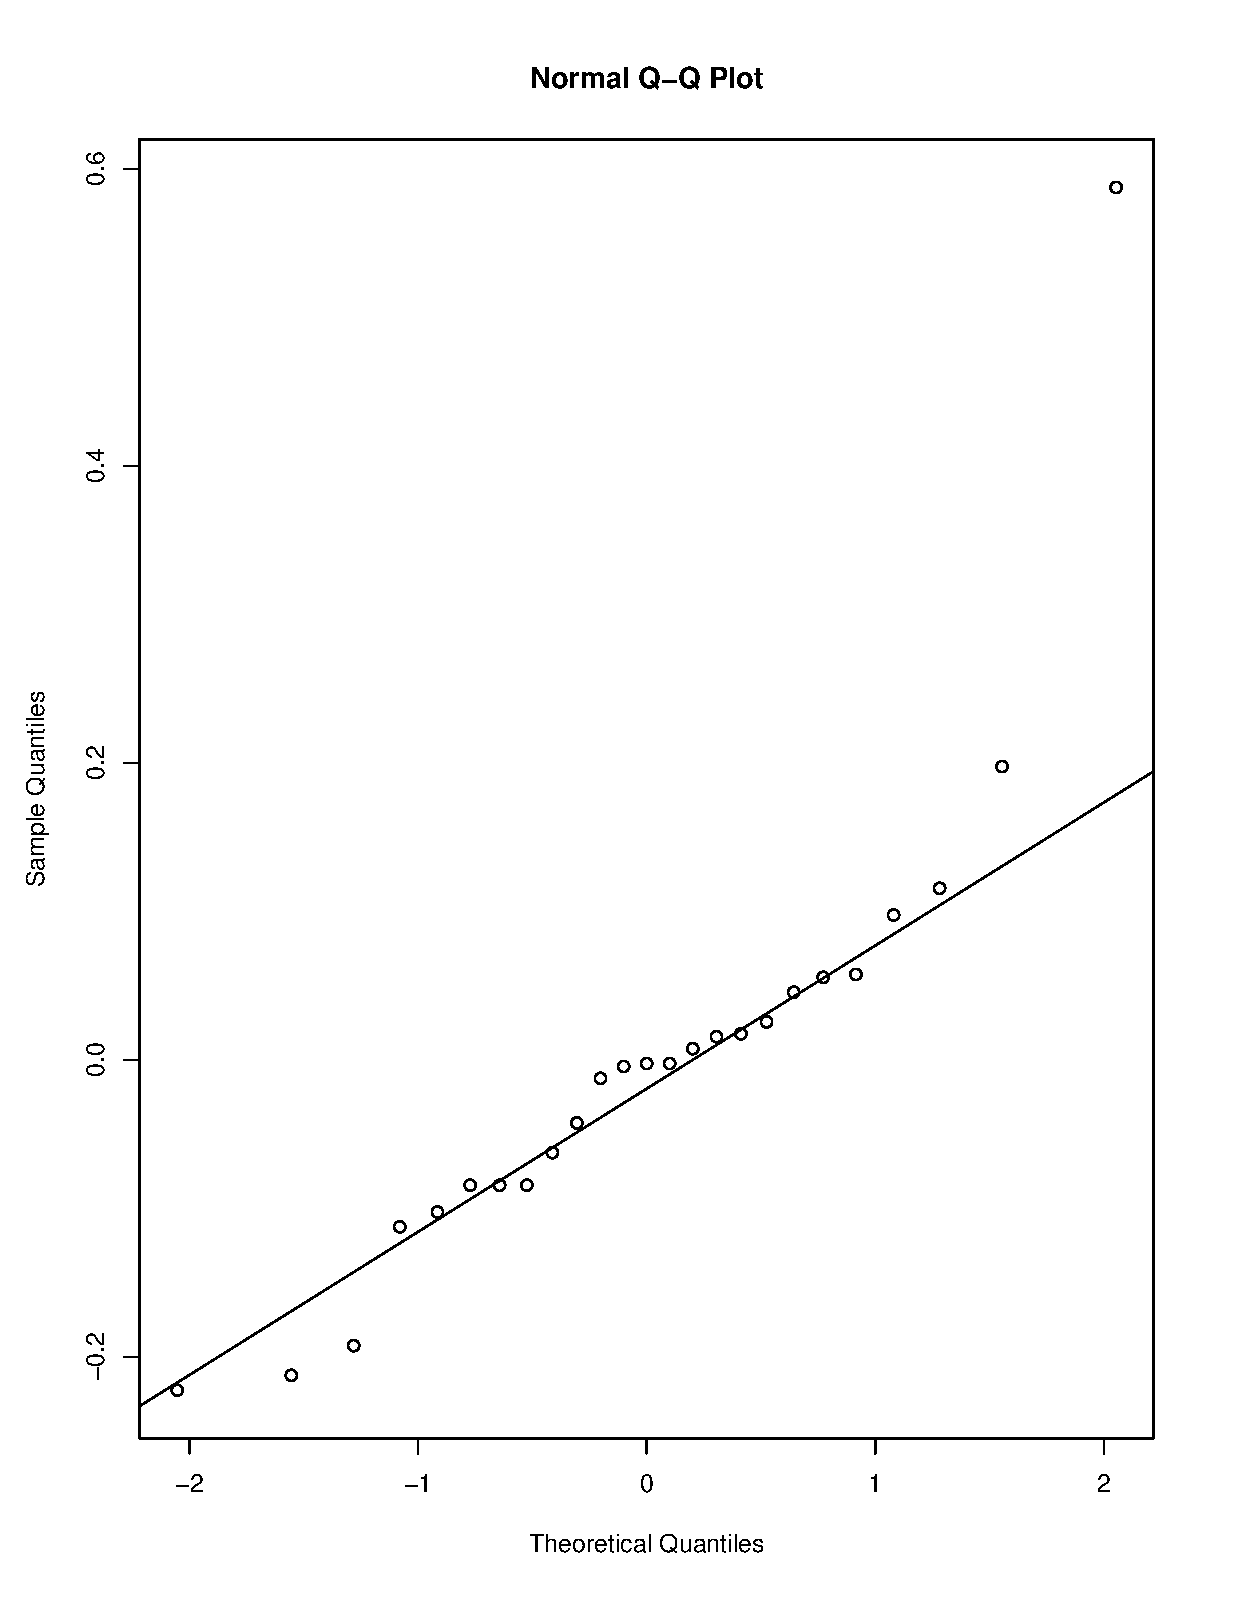
\includegraphics[width=0.7\textwidth]{qq}
  \caption{P1: q-q plot for residuals\label{fig:qq}}
\end{figure}

For the equal variance assumption, I use Bartlett's test. Here is the
output from R:

\begin{verbatim}
	Bartlett test of homogeneity of variances

data:  data.p1$CCK and data.p1$Disease 
Bartlett's K-squared = 11.2755, df = 2, p-value = 0.003561
\end{verbatim}

As we can see, variance is not equal. However, I found the following
opinion on the Internet:

``Hypothesis testing is the wrong tool to use to asses the validity of
model assumptions. If the sample size is small, you have no power to
detect any variance differences, even if the variance differences are
large. If you have a large sample size you have power to detect even
the most trivial deviations from equal variance, so you will almost
always reject the null. Simulation studies have shown that preliminary
testing of model assumption leads to unreliable type I errors.

Looking at the residuals across all cells is a good indicator, or if
your data are normal, you can use the AIC or BIC with/without equal
variances as a selection procedure.''

As a result, since the sample size is small, the unequal variance test
is not reliable. Therefore, we don't need to test the unequal
variance. \\

c) \\

The result from Kruskal-Wallis rank sum test is 

\begin{verbatim}
	Kruskal-Wallis rank sum test

data:  data.p1$CCK and data.p1$Disease 
Kruskal-Wallis chi-squared = 13.8673, df = 2, p-value = 0.0009744
\end{verbatim}

As we can see, both parametric and non-parametric methods reject the
null hypothesis.

\section*{Question 2}

a) \\

I use the two-way ANOVA to o do the analysis. Here is the output of
the F-test from R:

\begin{verbatim}
                  Df Sum Sq Mean Sq F value    Pr(>F)    
ADOPTIVE           1 1477.6 1477.63  8.4561 0.0063663 ** 
BIOLOGIC           1 2291.5 2291.47 13.1135 0.0009445 ***
ADOPTIVE:BIOLOGIC  1    1.9    1.91  0.0109 0.9174370    
Residuals         34 5941.2  174.74                      
---
Signif. codes:  0 ‘***’ 0.001 ‘**’ 0.01 ‘*’ 0.05 ‘.’ 0.1 ‘ ’ 1 
\end{verbatim}

And the coefficient is:

\begin{verbatim}
            (Intercept)             ADOPTIVELow             BIOLOGICLow 
                  119.6                   -12.1                   -16.0 
ADOPTIVELow:BIOLOGICLow 
                    0.9
\end{verbatim}

As we can see, there is no interaction term. And the SES of biological
parents effects larger than the SES of adoptive parents
$(16.0:12.1)$. \\

b) \\

For the normality assumption, we use q-q plot of residuals to do
the analysis. The plot is shown in Fig-\ref{fig:qq2}. As we can see,
the normality assumption holds.

\begin{figure}[ht!]
  \centering
  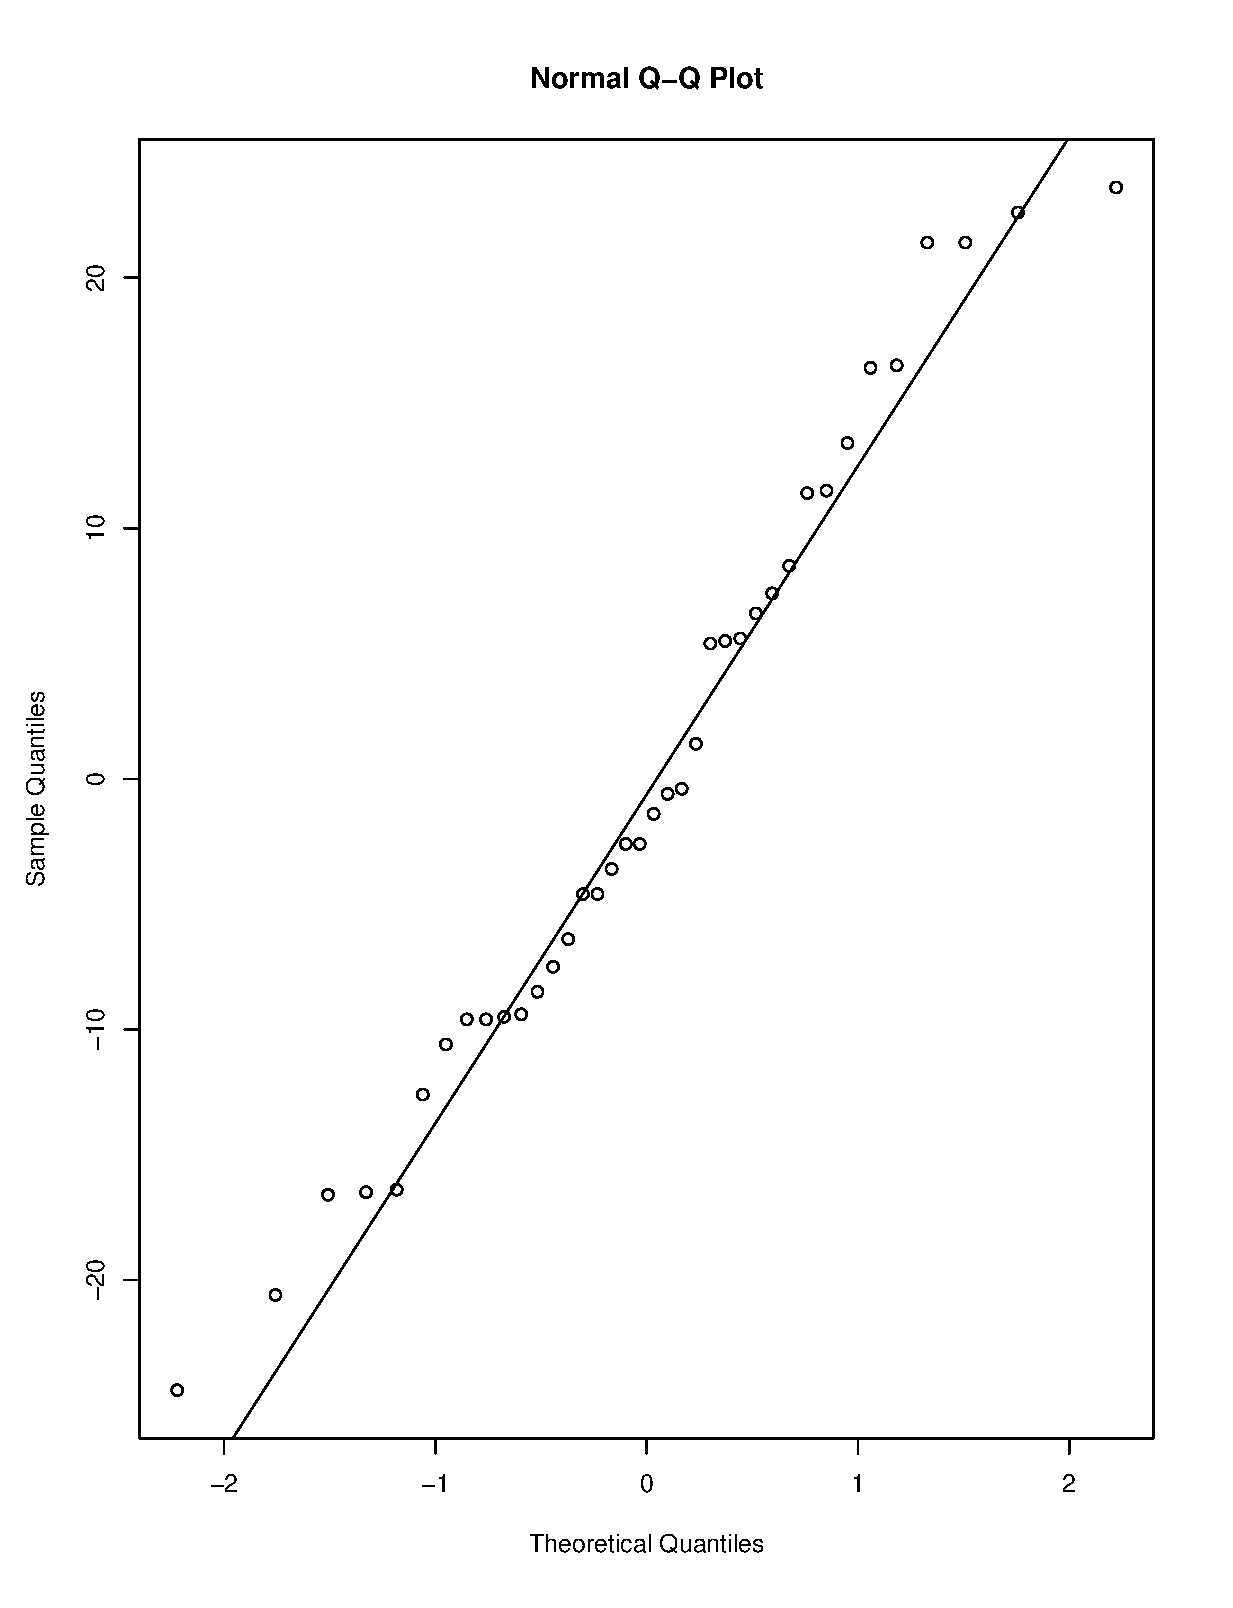
\includegraphics[width=0.7\textwidth]{qq2}
  \caption{P2: q-q plot for residuals \label{fig:qq2}}
\end{figure}

\appendix
\appendixpage
\addappheadtotoc

The R code is listed below:

\verbatiminput{hmwk7.r}

The MATLAB code is listed below:

\verbatiminput{hmwk7.m}

\end{document} 
